
\title{POM}

\documentclass[12pt]{article}
\newcommand{\reversecount}{
\begin{minipage}[t]{0.4\textwidth}
	\begin{itemize}
	\item Column 2 content 1
	\item Column 2 content 2
	\end{itemize}
\end{minipage}
}
\usepackage{import}
\usepackage{xifthen}
\usepackage{pdfpages}
\usepackage{transparent}
\usepackage{float}
\usepackage{tcolorbox}
\usepackage{amsmath}
\begin{document}

\maketitle

\section{Introduction to Marketing}

What is marketing? Well, one can talk about this in various different way, but let's start with the word itself.
$$ \text{Market}+\text{ing} $$

As the word implies, it can be seen as "doing the market", or, trying to be better with dealing markets. Therefore one can say that marketing is just

\begin{tcolorbox}
		\text{Any transaction between Producer and Consumer to Promote trading}
\end{tcolorbox}

That makes marketing to be seen as "Trading Obstacles Elimination" Therefore, making 4 possible following tasks
\begin{itemize}
	\item Make product that consumer wants
	\item Make it noticeable by people
	\item Solve the possible causes that make buying difficult.
	\item Keep the continual trading relationship.
\end{itemize}

Overall, we want the management system to sustain these tasks
\begin{figure}[ht]
	\centering
	\def\svgwidth{\columnwidth}
	\import{./figures/}{test.pdf_tex}
	\caption{test}
	\label{fig:test}
\end{figure}
% \begin{figure}[H]
% 	\centering
% 	\def\svgwidth{\columnwidth}
% 	\import{./figures/}{marketingmanagement.pdf_tex}
% 	\caption{marketingmanagement}
% 	\label{fig:marketingmanagement}
% \end{figure}

C. SWOT analysis

1. Basic Model

BCG Model

The Purpose of BCG matrix: Set the balance of Cash Flow.
\begin{figure}[H]
	\centering
	\def\svgwidth{\columnwidth}
	\import{./figures/}{BCG.pdf_tex}
	\caption{BCG}
	\label{fig:BCG Model}
\end{figure}

Problem of BCG Model

\begin{itemize}
  \item Way too simple x, y cord.
  \item Vague definition of market.
  \item Vague borderline of MGR, H/L
  \item Considers only present state.
  \item Can be too drastic.
  \item Don't consider any synergic possibilities.
\end{itemize}

1) X as "Position of competition" Y as "Attractiveness of Business"

2) Define market within realm of SUB

3) High - Medium - Low

%9월 11일

\section{Marketing research}

\subsection{Topics of Marketing research}

1. Analyzing Situation step
\begin{itemize}
	\item Changes in Inside, outside Environments
	\item strength, weakness of our, opponent companies
	\item catching opportunities/analyzing market character
	\item analyzing consumers
\end{itemize}

2. Collecting strategies step
\begin{itemize}
	\item researching consumer's cognition
	\item market test (concept, elasticity of price, predict demand)
	\item
\end{itemize}

3. Strategies acquiring step
\begin{itemize}
	\item add tracking
	\item new product tracking (recognition, preference ... )
\end{itemize}

4. Evaluate step
market share, mind share, brand equity, satisfaction



How do we get the data?
\begin{enumerate}
	\item Search for it (online, researches...)
	\item Make them!
	\item Buy them! (or let other make them)
\end{enumerate}

\subsection{Marketing research process}

\begin{enumerate}
	\item Decide whether we need to research
	\item Specify why we need to research (What are you trying to get by this research?)
	\item type of Constructions of research
	\item Data Source (Do we make them? search for it? etc..)
	\item How do we collect our data?
	\item Extract samples and collect Data (what is our sample group? how? how many?)
	\item Analysis of our data
	\item Result and organize the product.
\end{enumerate}

\subsubsection{Type of research construction}
\begin{enumerate}
	\item Exploratory research
	\begin{itemize}
		\item "Why do we lack net profit?"
		\item "would single family's consuming mind different?"
	\end{itemize}
	\item Descriptive research (much more enumerative and analytical, more to correlational study)
	\begin{itemize}
		\item "Is the reason of lack of net profit differ by different areas?"
		\item "Is the single family consumer sentiment differ by different age?"
	\end{itemize}
	\item Causal research (not much correlational, more causality research)
	\begin{itemize}
		\item "Is price discount better than quantity discount?"
		\item "Is minimalization better than advancing?"
	\end{itemize}
%Class 4_: 오후 3시 50분 ~ 4시 20분 사이 (탐색, 기술, 인과 조사 설명들...)

\end{enumerate}
\subsubsection{Data source}
\begin{enumerate}
	\item Secondary Data
	\begin{itemize}
		\item Inside data (Business related data..)
	\end{itemize}
	\item Primary data
	\begin{itemize}
		\item survey, test
		\item observation, ...
	\end{itemize}
	\item New raw Data
	\begin{itemize}
		\item Purchase Data
		\item clickstream Data
		\item UCC, SNS Data
		\item Big data (3V's)
	\end{itemize}
\end{enumerate}

\subsubsection{Example: Coke or Pepsi?}

Pepsi Challenge

"New coke" blunder

Despite all the research, why did so many people hate New coke?

"are you sure that taste only comes with tongue?"

By doing fMRI study of brain, one can find out that while blind testing, VMPFC of brain was triggered, while drinking coke, DLPFC and Hippocampus was triggered.

\subsubsection{Method of collecting Data}

\begin{enumerate}
	\item collecting Method
	\begin{itemize}
		\item face-to-face/or not
		\item mail, phone
		\item online
		\item mobile
	\end{itemize}
	\item Sampling
	\begin{itemize}
		\item sampling frame
		\item method of sampling (random sampling/easy sampling)
		\item sampling size
	\end{itemize}
\end{enumerate}


\section{Consumer Behavior Analysis}
\subsection{consumer behavior analysis tool}
1. Understanding consumer
\begin{itemize}
	\item who?
	\item what would they want?
	\item How would they react?
	\item why?
\end{itemize}

2. Decision making step
\begin{enumerate}
	\item facing the problem
	\item searching for information
	\item look for alternative
	\item Buying the product
	\item Action after buying product (usage and feedback)

\end{enumerate}

who would face the problem? not exactly the one who uses. can be parent, related people... etc..
Who would search for alternative? Thus, above order can be done by all separate people.
The 2. can be questioned by 1. therefore 20 questions can arise in total. However, the 1. can be much more descriptive.

Personal traits can be influential to Decision steps. This can be,
\begin{itemize}
	\item Memory
	\item attitude.
	\item etc...
\end{itemize}

\subsection{Consumer Behavior's general characteristic}

However, every consumer is human, therefore behaves in very "generalizable" way. It is natural to think that people behave in calculative, rational way. But this turned out to be very wrong.

\begin{enumerate}
	\item Decision making method routinized
	\begin{itemize}
		\item Extensive problem solving (Searching for all possible solution)
		\item Limited problem solving
		\item Routinized behavior
	\end{itemize}
	\item Behaviors within relationships(Between other objective beings)
	\begin{itemize}
		\item Reference group influence (e.g. by pressure, I'm now fine with alcohol)
		\item Trickle down Effect
		There are differences between social hierarchy within behavior of consumers. So called "lower class" tends to follow "higher class"
		\item Social modeling (People tends to follow other people in general. especially who they admire)
		Why is it that, despite not believing the model is only working for "money", the influence is still there. This works for other examples not bounded by human models.
		\begin{figure}[H]
	\centering
	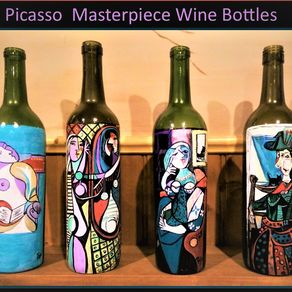
\includegraphics[width=0.95\textwidth]{img/picawine.png}
	\caption{Wine bottle with image of Picasso sells dramatically}
	\label{}
\end{figure}

	\end{itemize}
	\item Expected Irrationality (We are very irrational indeed, but we are irrational in very rational way. Therefore, pre-calculatable)
	\begin{itemize}
		\item Heuristics and biases
		\item  Emotional decisions
		\item Non conscious behaviors
	\end{itemize}
\end{enumerate}

How many of us make un-rational decisions? about 80\%, says our professor.


\end{document}
